\documentclass{beamer}
\usepackage[utf8]{inputenc}
%\usepackage{ngerman}
\usepackage{ulem}
\usepackage{color}
\usepackage{graphicx}
\usetheme{Copenhagen}
%\usetheme{Malmoe}
%\usepackage{pst-all}



%\useoutertheme{infolines}


\title[WIS]{Vorlesung Datenbanksysteme: \\ Praxisprojekt \\ Wahlinformationssystem \\ WS 2012/2013}
\author{Marcus Vetter, Sebastian Wöhrl}
\date{28. Januar 2013}

\begin{document}

\frame{\titlepage}

\begin{frame}
\frametitle{Wahlinformationssystem}
\begin{itemize}
\item System soll tabellarisch und graphisch eine Übersicht der Wahlergebnisse anzeigen
\item Ergebnis- und Analysedarstellung auf Wahlkreis- und Bundesebene
\item Webbasierte Abgabe von Erst- und Zweitstimmen (im Wahllokal)
\item System unterstützt die Verarbeitung mehrerer Bundestagswahlen
\end{itemize}
\end{frame}

\begin{frame}
\frametitle{Domänenmodell}
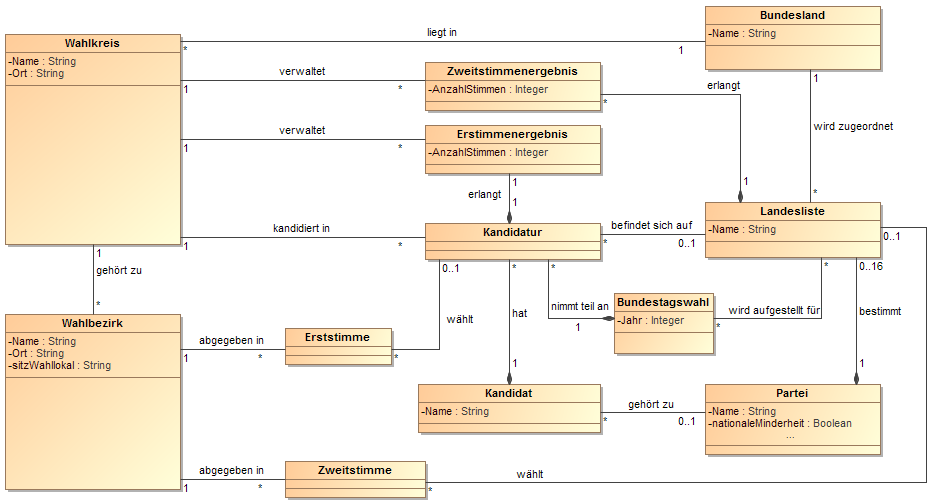
\includegraphics[scale=0.34]{cd_wahlinformationssystem.png}
\end{frame}


\begin{frame}
\frametitle{Architektur}
\begin{columns}
\begin{column}{7cm}
\begin{itemize}
\item Ergebnisberechnung vollständig in SQL
\item Webframework nur für Darstellung der Ergebnisse zuständig
\item Fachliche Logik so weit wie möglich in der Datenbank
\item Eingebautes Caching
\end{itemize}
\end{column}
\begin{column}{6cm}
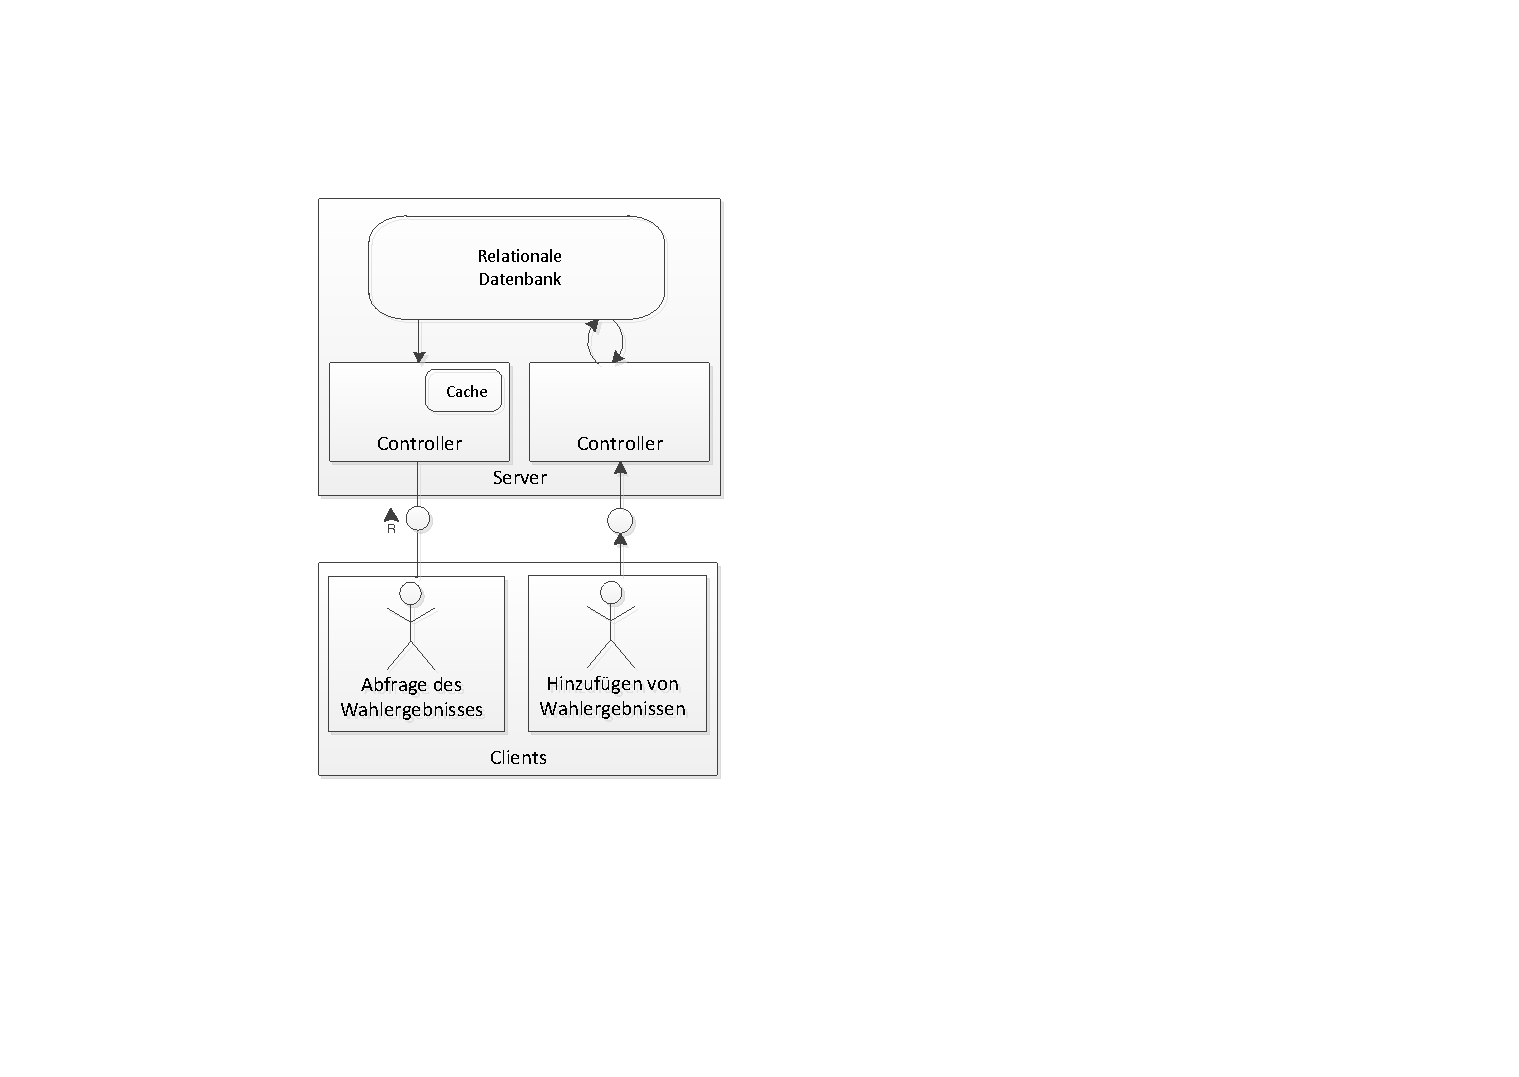
\includegraphics[scale=0.7]{Architecture.pdf}
\end{column}
\end{columns}
\end{frame}

\begin{frame}
\frametitle{Technische Grundlagen}
\begin{itemize}
\item Webbrowser-basiert
\item Playframework (Java / Scala)
\item Graphische Darstellung mit Google Charts API
\item PostgreSQL als Backend (Version 9.2)
\end{itemize}
\end{frame}


\begin{frame}
\frametitle{Vorführung}
\begin{center}
Live-Demo des Wahlinformationssystems
\end{center}
\end{frame}

\begin{frame}
\frametitle{}
\begin{center}
Vielen Dank für Ihre Aufmerksamkeit
\end{center}
\end{frame}


%\begin{frame}
%\frametitle{}
%\begin{itemize}
%\item 
%\end{itemize}
%\end{frame}



\end{document}